%!TEX root = shrink.tex


\section{\shrink\ design and implementation}
\label{sec:design}

Shrink is a system for server and network consolidation as well as load balancing. 
\shrink\ reduces a \cdc's energy use, while enabling operators to achieve the desired response times and hardware reliability.
A novel aspect of \shrink\ is its network-aware server consolidation scheme, which increases the energy savings that \shrink's network consolidation scheme achieves. This section describes \shrink's design goals, its design and its implementation.

\subsection{Design goals}
\shrink\  balances the following three requirements that are important from the perspective of a \cdc\ operator.

(1) \textbf{Energy use:} The design should minimize the energy use of a \cdc's servers and switches.

(2) \textbf{Response time:} The design should enable operators to provide the desired response time to end users. 

(3) \textbf{Hardware reliability:} The design should enable operators to achieve the desired hardware reliability, where reliability is quantified by the rate of on-off transitions for servers and switches. Note that a decrease in hardware lifetime due to frequent on-off transitions would result in the \cdc\ operator incurring greater capital expenditure over time. For example, if a hard disk rated at 50K start/stop cycles for reliable operation makes one on-off transition per hour, it reaches the start/stop cycles limit in 50K hours, much before its specified mean-time-before-failure of 1.2M hours \cite{seagate}.



\subsection{System overview}
\label{sec:overview}

\shrink\ runs as a control program that executes at fixed length intervals. In each interval, the control program receives  reports from all active servers regarding their load at the granularity of \emph{content buckets}; content are mapped to buckets using a consistent hash function based on their name.  
Based on three inputs  -- server load reports, a utilization vs. end-user response time curve for the operator's response time metric of interest (such as a given percentile of response time) and a specified value of end-user response time as per that metric -- , the control program computes the following two outputs: (1) \textbf{Consolidation:} The set of servers and switches to keep active, while remaining servers and switches are turned off. (2) \textbf{Load balancing:} A \emph{traffic split} for each bucket describing the ratio in which the bucket's requests are split among servers. We next describe \shrink's consolidation and load balancing algorithms, followed by how to compute the utilization vs. end-user response time curve provided to \shrink.
%
%
%server load reports, 
%
%
%
%a end-user response time metric specified by the operator (such as a given percentile of response time) and 
%
%

%\shrink\ runs as a control program that executes at fixed length intervals. In each interval, the control program receives  reports from all active servers regarding their load at the granularity of \emph{content buckets}; content are mapped to buckets using a consistent hash function based on their name.  Based on these server load reports, the control program computes the following two outputs: (1) \textbf{Consolidation:} The set of servers and switches to keep active, while remaining servers and switches are turned off. (2) \textbf{Load balancing:} A \emph{traffic split} for each bucket describing the ratio in which the bucket's requests are split among servers. Section \ref{sec:consolidation} and Section  \ref{sec:load-bal} describe the  \shrink's consolidation and load balancing algorithms respectively.


%, followed by how to compute the utilization-vs-response time curve provided to \shrink.


%\shrink\ seeks to minimize the number of servers and switches that are active under the following two constraints specified by an operator. (1) \emph{Server utilization limit} ($U$): \shrink\ keeps sufficient number of servers active so that the average load on active servers is less than this utilization limit. (2) \emph{Pre-shutdown wait interval} ($W$): \shrink\ turns servers off only after monitoring for the pre-shutdown wait interval that decrease in load is persistent rather than turning them off immediately. 

%Choosing the highest server utilization limit ($U$) that still achieves the desired end-user response times maximizes energy savings for operators. Unfortunately, the relation between $U$ and the response time  of \shrink\ is challenging to obtain without prior testing for a representative workload. To appreciate the challenge, consider this simple but  inaccurate way to select $U$. Given a desired response time ($r_0$) and the relation $r = f(u)$, which provides the steady-state response time $r$ of a server at an utilization $u$, choose $U = f^{-1}(r_0)$. The $U$ thus selected will likely result in a response time that is higher than the desired for several reasons such as imperfect load balancing, coordination overhead among peer caches and non-steady state behavior resulting from on-off transitions. The relation between $U$ and the response time of \shrink\ can be obtained with prior testing for a representative workload, thereby enabling operators to choose $U$ that maximizes energy savings while achieving desired response times.

%Choosing the smallest pre-shutdown wait interval ($W$) that still achieves the desired server reliability maximizes energy savings. With a smaller $W$, \shrink\  turns servers off sooner and saves more energy but potentially increases the rate of on-off transitions because of spurious decreases in load.   Our empirical results (Section \ref{sec:simulation})  show that $W$ in the range of 0.5-1 hr is a sweet spot for which energy use is 12-15\% higher than that achievable for a small value of $W$ = 1 min, and whose on-off transition rate is  nearly 10$\times$ lower than that of $W$ = 1 min. A similar analysis by operators for their workload can help choose $W$ that maximizes energy savings while achieving the desired server reliability.

%How does an operator select the utilization limit $U$ that maximizes energy savings while achieving the desired response time? A simple, but somewhat inaccurate, way to select $U$ is as follows. Given a desired response time ($r_0$) and a steady-state utilization-vs.-response time curve of a server $r = f(u)$, choose $U = f^{-1}(r_0)$. The utilization limit selected thus will likely result in a response time that is higher than the desired value due to imperfect load balancing and non-steady state behavior immediately after servers have been turned on or off. However, this utilization limit is expected to be a good starting point, after which operators can reduce $U$ in small decrements until response time reaches the desired value.

%The pre-shutdown wait interval determines the tradeoff between energy and reliability of servers. 



%

\subsection{Consolidation}
\label{sec:consolidation}
\shrink's consolidation algorithm assumes a datacenter topology in the form of a multi-rooted tree in which a topological ordering of nodes from left to right is well-defined at each level in the topology.  Servers and switches reside at leaf and non-leaf nodes respectively; root nodes provide external connectivity. To adapt network routing in response to network consolidation, \shrink\ requires the support for ECMP \cite{hopps2000analysis}, which is commonly available in the datacenter network fabrics today. 
%\TBD{why ecmp?}


\subsubsection{Server consolidation}
\label{sec:serverconsolidation}


%\begin{figure}[t]
%\centering
%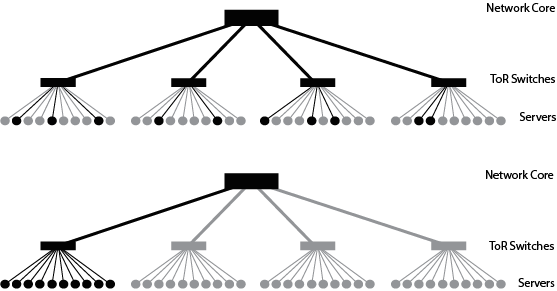
\includegraphics[scale=0.4]{figures/dcTopology.png}
%\caption{A datacenter topology. Black (grey) components are turned on (off). 
%(Top) Randomly choosing the set of active servers results in all ToR switches being turned on.
%(Bottom) Choosing the same number of active servers in a ``network-aware" manner enables more ToR switches to be turned off.}
%\label{fig:server-network}
%\end{figure}

%\shrink\ provides the following two parameters to operators to achieve the desired energy, performance and reliability: (1) \emph{Server utilization limit} ($U$): \shrink\ keeps sufficient number of servers active so that the average load on active servers is less than this utilization limit. (2) \emph{Pre-shutdown wait interval} ($W$): \shrink\ turns servers off only after monitoring for the pre-shutdown wait interval that decrease in load is persistent rather than turning them off immediately.

\shrink\ selects the active servers, in a network-aware manner, to be the leftmost leaf nodes in a topology. Figure \ref{fig:topo} shows why such a network-aware server consolidation can increase the energy savings that network consolidation achieves. In the figure, both the left and the right topologies  have 20 active servers.  The right topology requires all ToR switches to be kept active, but in the left topology the set of active servers are chosen among servers in one rack, which allows ToR switches in other racks to be turned off.  This example shows that consolidating servers in a network-aware manner can reduce network energy use.

\newcommand{\minServers}{\textit{minServers}}
\newcommand{\maxServers}{\textit{maxServers}}

Let $F(u)$ be the utilization vs. end-user response time curve for the operator's response time metric of interest provided to \shrink. $F(u)$ is similar to the end-to-end response time $(f(u) + mB + A)$ described in Section \ref{sec:analysis}. We discuss how $F(u)$ can be obtained in Section \ref{sec:utilization-vs-responsetime}.  \shrink\ uses $F(u)$ assuming that if the servers active in the datacenter are run at an average utilization $u$, then the resulting response time is $F(u)$. Thus, to achieve a specified end-user response time $R$, \shrink\ chooses a server utilization limit $U = r^{-1}(R)$.

%\shrink\ chooses a server utilization limit $U$ to achieve a specified end-user response time $R$.  If $F(u)$ is the utilization vs. end-user response time curve provided, $U = r^{-1}(R)$. $F(u)$ is similar to the end-to-end response time $(f(u) + mB + A)$ described in Section \ref{sec:analysis}. We discuss how $F(u)$ can be obtained in Section \ref{sec:utilization-vs-responsetime}. 

\shrink\ computes the number of active servers using two integer values: \minServers\ and \maxServers. \minServers\ $= \lceil L/U \rceil$, where the $L$ is the predicted load for the next interval; $L$ is predicted using linear regression based on the total load across servers in the past few intervals (default = 10 intervals). \maxServers\ is the maximum value of \minServers\ over the previous time window of length $W$; $W$ is called the \emph{pre-shutdown wait interval}. If \minServers\ $ > n$, where $n$ is the current number of active servers, $(\minServers\ - n)$ more servers are turned on, else if  \maxServers\ $ < n$,  $(n - \maxServers)$ servers are turned off.  

%the minimum and the maximum number of active servers denoted by \minServers\ and \maxServers\ respectively. 


\textbf{Reliability of servers:} The reliability of servers depends on the pre-shutdown wait interval ($W$). With a smaller $W$, \shrink\  turns servers off sooner and saves more energy but potentially increases the rate of on-off transitions because of spurious decreases in load.   Our empirical results (Section \ref{sec:simulation})  show that $W$ close to 1 hr is a sweet spot for which energy use is 15\% higher than that achievable for a small value of $W$ = 1 min, and whose on-off transition rate is  nearly 10$\times$ lower than that of $W$ = 1 min. Thus, we expect the default value of $W$ = 1 hr to work well for operators. However, operators can better inform their choice of $W$ with similar tests for their workload.

%Choosing the smallest pre-shutdown wait interval ($W$) that still achieves the desired server reliability maximizes energy savings. 

%The server consolidation algorithm runs periodically and calculates the minimum number of active servers using \minServers\ $ = \lceil L/U \rceil$, where $U$ is the server utilization limit and $L$ is the predicted load for the next interval. $L$ is predicted using linear regression based on the total load across servers in the past few intervals (default = 10 intervals). \shrink\ also computes  \maxServers, which is the maximum value of  \minServers\ across all the previous intervals in a time window of length $W$, which is the pre-shutdown wait interval. If \minServers\ $ > n$, where $n$ is the current number of active servers, $(\minServers\ - n)$ more servers are turned on, else if  \maxServers\ $ < n$,  $(n - \maxServers)$ servers are turned off. 




\subsubsection{Network consolidation}
\label{sec:node-selection}

\begin{figure}[t]
\centering
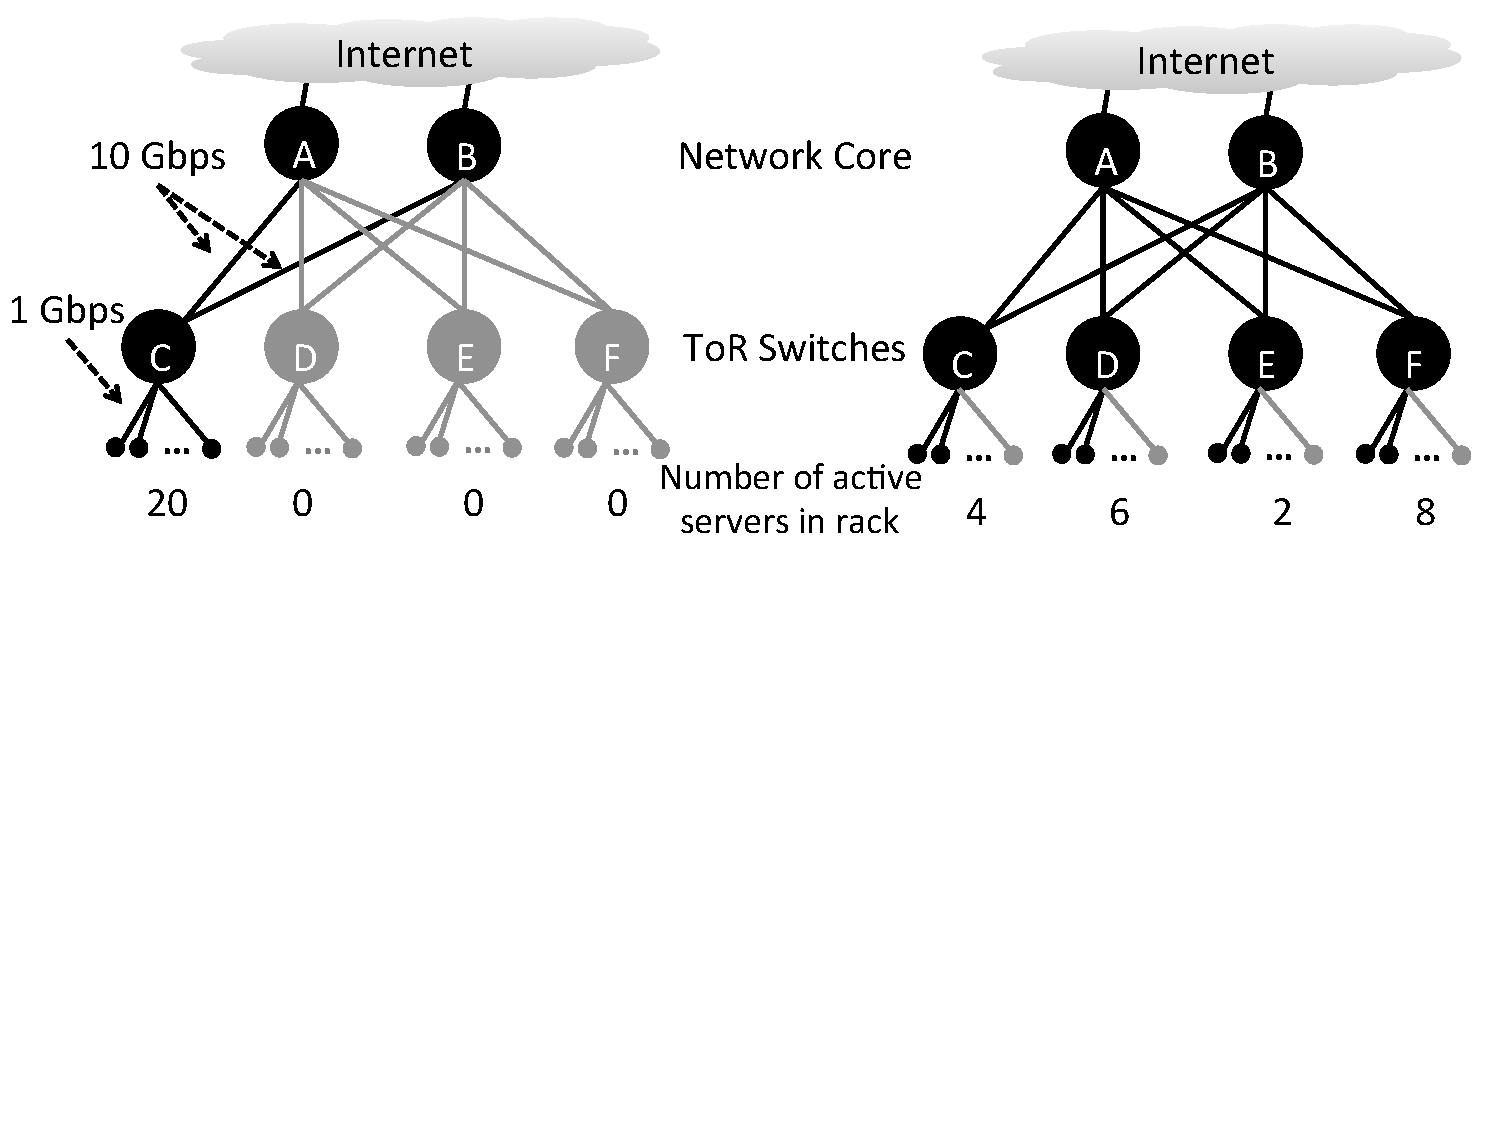
\includegraphics[scale=0.33]{figures/min-bw-v2.pdf}
\vspace{-1.4in}
\caption{Black (grey) components are turned on (off). Each rack has 20 servers. (Right) Randomly choosing the set of active servers results in all ToR switches being turned on. (Left) Choosing the same number of active servers in a ``network-aware" manner enables more ToR switches to be turned off.}
\label{fig:topo}
\end{figure}

%In a multi-rooted tree topology, we define the \emph{oversubscription ratio} as the total capacity of the links between the leaf nodes and the higher-level nodes in the topology and the total capacity of the links between the root nodes and the lower-level nodes in the topology.

Network consolidation in \shrink\ satisfies the following condition: assuming ECMP routing, all active servers can simultaneously send traffic to clients equal to the \emph{external bandwidth} using the set of active switches only. We define the external bandwidth as the outgoing link capacity of a server divided by the oversubscription ratio of the datacenter. For example, in a network with 2:1 oversubscription and 1 Gbps server outgoing links, the external bandwidth is 500 Mbps. If a server sends traffic at a maximum rate up to the external bandwidth, then this condition avoids network bottlenecks.  

We explain the above observation using an example. Consider the topology in Figure \ref{fig:topo} (left) in which the external bandwidth is 1 Gbps. Let us assume that only servers connected to switch C are active due to consolidation. Let the maximum rate of traffic from a server to clients be 800 Mbps. If all active servers are sending traffic at their maximum rate, then the total traffic from switch C to core switches A \& B is (800 Mbps)$\times$20 = 16 Gbps. If both A \& B are active, the condition above is satisfied, and all servers can simultaneously send traffic  to clients at their maximum rate. If  A is on but B is off, the condition above is not satisfied, and as a result, a network bottleneck happens on link AC.

\eat{
\begin{algorithm}[t]\small
  \SetAlgoLined
  \SetKwInOut{Input}{input}
  \SetKwInOut{Output}{output}
\Input{$V$ \textit{// set of servers and switches}}
\Input{$S$ 	\emph{// set of active servers}}
\Output{$R$ 	\emph{// set of active switches}}
$T$ = \{\} 	\emph{// traffic sent towards root by each node}\\
\For{ $v \in V$}{
	$T[v]$ = $(v \in S)$ ? external bw : 0\\
}
$H$ = height of tree topology \emph{// leaves have height 1}\\
\For{ $h = 1\ \KwTo\ (H - 1)$}{
	$V_h$ = list of nodes at height $h$ in left to right order\\
	\For{ $v \in V_h$}{
		\If{$ T[v] > 0$}{
			$L$ = link capacity from switch $v$ to any parent\\
			$P$ = list of $\lceil T[v]/L \rceil$ leftmost parents of node $v$\\
			\For{ $p \in P$}{
				$T[p] = T[p] + T[v]/(\lceil T[v]/L\rceil)$\\ 
				$R = R \cup \{p\}$  \emph{// Parent p must be active}\\
			}
		}
	}
}
\caption{Network consolidation}
\label{algo:network}			
\end{algorithm}
}

%\shrink's network consolidation  assumes that each active server is sending traffic to clients at a rate equal to the external bandwidth. It selects the set of switches that are needed to route this traffic to the root nodes. It considers switches in the order of increasing height and among switches at the same height considers them in a left-to-right order. Each switch selects the $k$-leftmost parents, where $k$ is the least value for which the sum of capacities of links to the selected parent nodes is equal or more than than the traffic sent by the switch's child nodes; the switch then forwards the traffic sent by its children among its selected parents equally.  At the end, only the switches that are transmitting non-zero traffic are selected to be active.

\shrink's network consolidation assumes that each active server is sending traffic to clients at a rate equal to the external bandwidth. It selects the set of switches needed to route this traffic to the root nodes. It considers switches in the order of increasing height from leaf to root and among switches at the same height considers them in a left-to-right order. Each switches selects $p$-leftmost parents that must be active to forward the traffic sent by its children to root nodes; $p$ is the least value for which the sum of capacities of links to the selected parent nodes is equal or more than than the traffic sent by the switch's child nodes. Due to ECMP support, traffic forwarded to root nodes is divided on links to the $p$ parent nodes equally.
Finally, only the switches that are transmitting non-zero traffic are selected to be active.




\textbf{Reliability of switches:} Network consolidation in \shrink\ satisfies the following property related to reliability of switches: if the number of active servers increases, additional servers and switches are turned on, but none of the servers and switches that are already active are turned off. Due to this property,  the rate of on-off transitions of switches is close to that of on-off transitions for servers. For example, consider a time interval in which the number of active servers is monotonically increased from $1$ to $N$, where $N$ is the total number of servers. In this interval, there is at most one transition from off to on state for each server. Due to the above property, the set of active switches can only add new switches as the number of active servers increases. As a result, each switch would also have at most one transition from off to on state in this interval. Thus, the above property ensures that improving server reliability improves switch reliability as a consequence.

\newcommand{\B}{\textit{buckets}}
\newcommand{\Load}{\textit{bktsLoad}}
\newcommand{\Srvrs}{\textit{srvrs}}
\newcommand{\U}{\textit{U}}
\newcommand{\kcnt}{\textit{k}}
\newcommand{\TS}{\textit{trSplits}}
\newcommand{\TSNEW}{\textit{newTrSplits}}
\newcommand{\limit}{\textit{limit}}
\newcommand{\D}{\textit{srvrsLoad}}
\newcommand{\BNEW}{\textit{newTrSplitBkts}}
\newcommand{\R}{\textit{bktTrSplit}}
\newcommand{\bkt}{\textit{bkt}}
\newcommand{\lrem}{\textit{remBktLoad}}
\newcommand{\srvr}{\textit{srvr}}
\newcommand{\smin}{\textit{minLoadSrvr}}
\newcommand{\load}{\textit{load}}

\begin{algorithm}[t]\small
  \SetAlgoLined
  \SetKwInOut{Input}{input}
  \SetKwInOut{Output}{output}
\Input{\B\ \textit{// set of content buckets}}
 \SetKwInOut{Input}{}
\Input{\Load\ \textit{// content bucket to load map}}
\Input{\Srvrs\ 	\textit{// set of active servers}}
\Input{\U\ 	\textit{// server utilization limit}}
\Input{\kcnt\ 	\textit{// default server count serving a content bucket}}
\Input{\TS\ \textit{// bucket to traffic split  map (old)}}
\Output{\TSNEW\ \textit{//  bucket to traffic split map (new)}}
\limit = max($\frac{\sum_{\bkt \in \B}{\Load[\bkt]} }{|\Srvrs|}$, \U) \textit{// server load limit}\label{st:maxload}\\
\D\ = \{\} \textit{// server to load map}\\
\For{\srvr $\in$ \Srvrs}{\D[\srvr]\ = 0}
\BNEW\ = \{\} \textit{// buckets needing new traffic splits}\\
\For{\bkt\ $\in$ \B}{
	\For{$(s_j^{\bkt}, f_j^{\bkt}) \in \TS[{\bkt}]$} {
		\textit{// server $s_j^{\bkt}$ serves a fraction $f_j^{\bkt}$ of {\bkt}'s load}\\
		\If{$s_j^{\bkt} \notin \Srvrs$ or  $\D[s_j^{\bkt}] + f_j^{\bkt}\Load[{\bkt}] > \limit$}{
			Add \bkt\ to \BNEW\ \\
			\textbf{break}\\
		}
	}
	\If{$\bkt\ \notin$ \BNEW}{
		\For{$(s_j^{\bkt}, f_j^{\bkt}) \in \TS[{\bkt}]$} {
			$\D[s_j^{\bkt}]\ += f_j^{\bkt}\Load[{\bkt}]$
		}
		$\TS[\bkt] = \TSNEW[{\bkt}]$ \\
	}

}

\For{ \bkt\ $\in $ \BNEW}{
	select \kcnt\ servers $(s_1, s_2, ... s_{\kcnt})$ randomly from \Srvrs\\
	\R = \{\} \textit{// new traffic split for \bkt\ }\\
	\lrem\ = \Load[\bkt]  \textit{// remaining load for \bkt\ }\\
	\For{\srvr\ $\in (s_1, ... s_{\kcnt})$} {
		\If{\D[\srvr] + \Load[\bkt]/\kcnt\ $<$ \limit} {
			\R\ = \R\ $\cup$ \{(\srvr, 1/\kcnt)\}\\
			\lrem\ $-=$  \Load[\bkt]/\kcnt\\ 
		}
	}
	\While{\lrem\ $>$ 0} {
		select \smin\ whose  \D[\smin] is the least\\
		\load\ = min(\lrem, \limit\ $-$ \D[\smin])\\
		\lrem\ $-=$ \load\\
		Add 	\{(\smin, $\frac{\load}{\Load[\bkt]}$)\} to \R \\
		%\R\ = \R\ $\cup$ \{(\smin, \load/\Load[\bkt])\} \\
	}
	\TSNEW[\bkt] = \R\ \\
}

\caption{Load balancing}
\label{algo:lb}			
\end{algorithm}

%
%\begin{algorithm}[t]\small
%  \SetAlgoLined
%  \SetKwInOut{Input}{input}
%  \SetKwInOut{Output}{output}
%\Input{$B$ \textit{// set of content buckets}}
% \SetKwInOut{Input}{}
%\Input{$L$ \textit{// map from content bucket to load}}
%\Input{$S$ 	\textit{// set of active servers}}
%\Input{$U$ 	\textit{// server utilization limit}}
%\Input{$k$ 	\textit{// default server count serving a content bucket}}
%\Input{\textit{TS} 	\textit{// old map from bucket to traffic split}}
%\Output{\textit{TS\_NEW} 	\textit{// new map from bucket to traffic split}}
%\textit{lim} = max ($\sum_{i \in B}{L[i]}/|S $, $U$) \textit{// load limit for a server} \label{st:maxload}\\
%$D = \{\}$ \textit{// map from server to load}\\
%\For{$s \in S$}{$D[s] = 0$}
%\textit{B\_NEW} = \{\} \textit{// set of buckets needing new rules}\\
%\For{$ i \in B$}{
%	\For{$(s_j^i, f_j^i) \in P[i]$} {
%		\textit{// server $s_j^i$ serves a fraction $f_j^i$ of bucket $i$'s load}\\
%		\If{$s_j^i \notin S$ or  $D[s_j^i] + f_j^iL[i] > \textit{lim}$}{
%			\textit{B\_NEW} =  \textit{B\_NEW} $\cup$ \{i\}\\
%			\textbf{break}\\
%		}
%	}
%	\If{$i \notin$ \textit{B\_NEW}}{
%		\For{$(s_j^i, f_j^i) \in P[i]$} {
%			$D[s_j^i] = D[s_j^i] + f_j^iL[i]$
%		}
%		$\textit{TS}[i] = \textit{TS\_NEW}[i]$ \textit{// traffic split unchanged}\\
%	}
%
%}
%
%\For{$ i \in $ \textit{B\_NEW}}{
%	select $k$ servers $(s_1^i, s_2^i, ... s_1^k)$ randomly from $S$\\
%	$R$ = \{\} \textit{// new traffic split for bucket $i$}\\
%	\textit{l\_rem} = $L[i]$  \textit{// remaining load for bucket $i$}\\
%	\For{$s_j^i \in (s_1^i, ... s_1^k)$} {
%		\If{$D[s_j^i] + L[i]/k < \textit{lim}$} {
%			$R = R \cup \{(s_j^i, 1/k)\}$\\
%			$\textit{l\_rem} = \textit{l\_rem} +  L[i]/k$\\ 
%		}
%	}
%	\While{\textit{l\_rem} $>$ 0} {
%		select server \textit{s\_min} whose load  $D[\textit{s\_min}]$ is the least\\
%		$l$ = min(\textit{l\_rem}, \textit{lim} - $D[\textit{s\_min}]$)\\
%		$\textit{l\_rem} = \textit{l\_rem} - l$\\
%		$R = R \cup \{(\textit{s\_min}, l/L[i]) \} $\\
%	}
%	\textit{TS\_NEW}[i] = $R$ \textit{// traffic split updated for bucket $i$}\\
%}
%
%\caption{Load balancing}
%\label{algo:lb}			
%\end{algorithm}


\subsection{Load balancing}
\label{sec:load-bal}
\shrink\  uses randomized load balancing over a set of content buckets. Content is mapped to a fixed number of buckets (default = 100) using a consistent hash function based on its name. The output of load balancing is a \emph{traffic split} for each bucket that determines the ratios in which the bucket's requests will be distributed among \cdc's servers. Traffic split for a bucket is determined based on the load predicted for the bucket in the next interval. \shrink\ predicts a bucket's load using a linear regression model trained based on the observed load for the bucket in the past few intervals.

\shrink's load balancing (Algorithm \ref{algo:lb}) selects a load limit for servers, which is greater of the server utilization limit $U$ or the average load on an active server (line \ref{st:maxload}). The algorithm selects buckets that need new traffic splits compared to the previous execution of the algorithm. These buckets either belong to servers that are no longer active or whose load exceeds the  load limit (lines 5-15). 
To compute new traffic splits for the selected buckets, \shrink\ selects a fixed number of randomly chosen servers (default = 2)  and divides the load for the bucket among them equally. In doing so, if the load on any server exceeds the load limit then \shrink\ assigns the excess load for that bucket from that server to the least loaded server that is active (lines 16-29). 

Load balancing mitigates disruptions to the existing connections by not sending requests to a server that is likely to be turned off. To this end, \shrink's node selection module informs the load balancing module that a server is likely to be turned off in the middle of the pre-shutdown wait interval of the server. As the pre-shutdown wait interval is tens of minutes long, existing connections, except for the long transfers, complete before server shutdown. To mask the server turnoff for these few long transfers, \cdc s can use techniques such as  IP address takeover \cite{flickenger2003linux} or connection migration across machines \cite{snoeren2001fine,sultan2002migratory}. We have not implemented these techniques in \shrink.

\subsection{Computing utilization vs. response time curve}
\label{sec:utilization-vs-responsetime}

We discuss three ways of computing the utilization vs. response time curve $F(u)$ input to \shrink\ in the order of increasing complexity. The more complex schemes potentially enable \shrink\ to provide response times that are closer to those specified by operators. 

The first and second approaches require prior measurements of a single server and of the entire \cdc\ respectively.
These measurements obtain the  value of the operator's response time metric of interest at varying levels of utilization.  These measurements are done with a representative workload in a test environment with real or emulated client-to-server delay and server-to-origin delay.  The first approach implicitly assumes that if the response time of a single server at utilization $u$ is $r$, then the response time of the \cdc\ whose servers have an average utilization $u$ is also $r$. This assumption ignores the inefficiencies of a distributed system such as imperfect load balancing and coordination overhead among peer caches in a \cdc. These factors are more accurately accounted for in the second approach. Nonetheless, both approaches could be inaccurate as they do not consider the non-steady cache behavior due to on-off transitions and increased cache miss rates due to reduced storage.  To account for these inaccuracies, a constant inefficiency factor $\rho$ is added as follows. If $F'(u)$ is the measured  utilization vs. response time curve, then \shrink\ is input a curve $F(u) = \rho \times F'(u)$.

The third approach is to equip \shrink\ to learn the curve automatically based on online measurements. The overhead of these measurements can be kept small by doing them for a small fraction of requests only. This approach could be more accurate than the previous two approaches because it considers the factors discussed above and can even adapt to changes in workload characteristics that influence the utilization vs. response time behavior. We have not implemented this third approach in \shrink. 





%We discuss three ways of computing the utilization vs. response time curve that is provided to \shrink\ in the order of increasing complexity. The more complex schemes potentially enable \shrink\ to provide response times that are closer to those specified by operators. The first and second approaches require prior measurements at varying levels of utilization of a single server and of the entire \cdc\  respectively. Similar to to the assumption made in deriving the model in Section \ref{sec:analysis}, the first approach implicitly assumes that the utilization vs. response time behavior of the datacenter is the same as that of a single server. However, a \cdc\ will likely have a higher response time than a single server at the same utilization because imperfect load balancing and coordination overhead among peer caches in a \cdc.  These factors are accounted for in the second approach; therefore, its utilization vs. response time curve is closer to the actual curve than the first approach.

%The first, and the simplest, approach is to compute the utilization vs. response time curve based on profiling a single server at varying levels of utilization. This approach implicitly assumes that the utilization vs. response time behavior of the datacenter is the same as that of a single server; we make the same assumption in Section \ref{sec:multiserver}. 

%The second approach is to compute the curve by profiling the entire \cdc\ at varying levels of utilization. 



\subsection{Implementation}
\label{sec:implement}
Our \shrink\ prototype is implemented in nearly 6K lines of  Java code. By default, \shrink's control program runs at 20 sec intervals. Shrink uses Squid as a caching proxy \cite{squid}. We configured Squid to use its AUFS storage, which handles disk accesses asynchronously by multiple threads; AUFS results in lower response over synchronous disk access storage mechanisms. We have added  support for content chunking in order to reduce origin traffic and improve cache hit rates: specifically, a large file is requested as a sequence of 2 MB chunks, which enables Squid to cache each chunk independently.

\textbf{Load balancing:} \shrink\ resembles a DNS load balancer. Similar to a DNS resolution, a client contacts \shrink\ to receive the traffic split for a content, and then the client contacts a server as per the traffic split to download the content. 
An alternative would have been to implement \shrink\ as a middlebox. As a middlebox routes the traffic between clients and servers through it, it would have become a network bottleneck on our testbed. In comparison, a DNS-type load balancer does not become a network bottleneck as it only exchanges load balancing queries and responses from clients. 

\textbf{Server load measurement:} We measure a server's load in terms of request rates.  We use an approach that requires no modification to the Squid codebase. We run a process on each server that parses the content access logs output by Squid, and sends to \shrink, once every interval, the number of requests for each content bucket at that server in the previous interval.

\textbf{Peer caching overhead:} Each Squid instance runs as an independent cache that fetches content from origin servers upon a cache miss. We tested a configuration of Squid in which all servers were configured as cache peers that used Internet Cache Protocol (ICP) \cite{wessels1997rfc} for querying peer caches upon a cache miss. But, we found the overhead of  ICP to be nearly 25\% of the overall request load while the peer cache hits were less than 3\%. Hence, we disabled ICP due to its lower benefit compared to its overhead.

%\textbf{Content chunking:} 

A limitation of our prototype is the lack of power controls for servers and switches. We emulate the startup (shutdown) delay of servers by waiting for a pre-defined interval before  restarting (killing) the server-side processes.  Finally, we note that remote power management that is necessary for turning servers and switches on and off is available from multiple vendors today \cite{s-power,s2-power}.


